%-----------------------------------------------------------------------------
\section{DSP em Arduino}
%-----------------------------------------------------------------------------


\subsection{Entrada de áudio: ADC}

%-----------------------------------------------------------------------------
\begin{frame}{Conversor analógico-digital (ADC)}
Características do ADC no ATmega328P:
\begin{itemize}
  \item Amostragem:
    \begin{enumerate}
      \item \emph{Sample and hold}.
      \item Aproximação sucessiva.
    \end{enumerate}
  \item Resolução: 8 ou 10 bits.
  \item Tempo de conversão: 13 a 260 $\mu$s.
  \item Frequência própria / redução de ruído.
  \item Conversão manual ou automática.
\end{itemize}
\end{frame}
%-----------------------------------------------------------------------------

%-----------------------------------------------------------------------------
\begin{frame}{Conversor analógico-digital (ADC)}
Medição do tempo de conversão, usando diferentes valores de pré-escalonador
(frequência principal: 16~MHz):
\begin{center}
\begin{tabular}{crrrr}
\toprule
\toprule
\footnotesize{pré-escalonador} & \footnotesize{$f_\text{ADC}$ (KHz)} &
\footnotesize{$T_\text{ADC}$ ($\mu$s)} & \footnotesize{$\tilde{T}_\text{conv}$ ($\mu$s)} & \footnotesize{$\tilde{f}_\text{conv}$ ($\approx$Hz)} \\
\midrule
2 & 8.000 & 0,125 & 12,61 & 79.302\\
4 & 4.000 & 0,25 & 16,06  & 62.266 \\
\rowcolor{LightCyan}
8 & 2.000 & 0,50 & 19,76  & 50.607 \\
16& 1.000 & 1 & 20,52  & 48.732 \\
32& 500 & 2 & 34,80  & 28.735 \\
64& 250 & 3 & 67,89  & 14.729 \\
128& 125 & 8 & 114,85 & 8.707  \\
\bottomrule
\end{tabular}
\end{center}
Obs:
\begin{itemize}
  \item Resolução da função \texttt{micros()}: 4~$\mu$s.
  \item Período de conversão: $\approx$ $14,5 \times T_\text{ADC}$. 
  \item $R=44.100$~Hz $\Rightarrow$ $T_\text{amostra} \approx 22,67~\mu$s.
  \item $R=31.250$~Hz $\Rightarrow$ $T_\text{amostra} = 32,00~\mu$s.
\end{itemize}
\end{frame}
%-----------------------------------------------------------------------------

%-----------------------------------------------------------------------------
\begin{frame}{Conversor analógico-digital (ADC)}
Parâmetros escolhidos:
\begin{itemize}
  \item Conversão alinhada à esquerda (8 bits).
  \item Pré-escalonador igual a 8.
\end{itemize}
\end{frame}
%-----------------------------------------------------------------------------

\subsection{Saída de áudio: PWM}

%-----------------------------------------------------------------------------
\begin{frame}{Modulação por largura de pulso (PWM)}
\begin{figure}
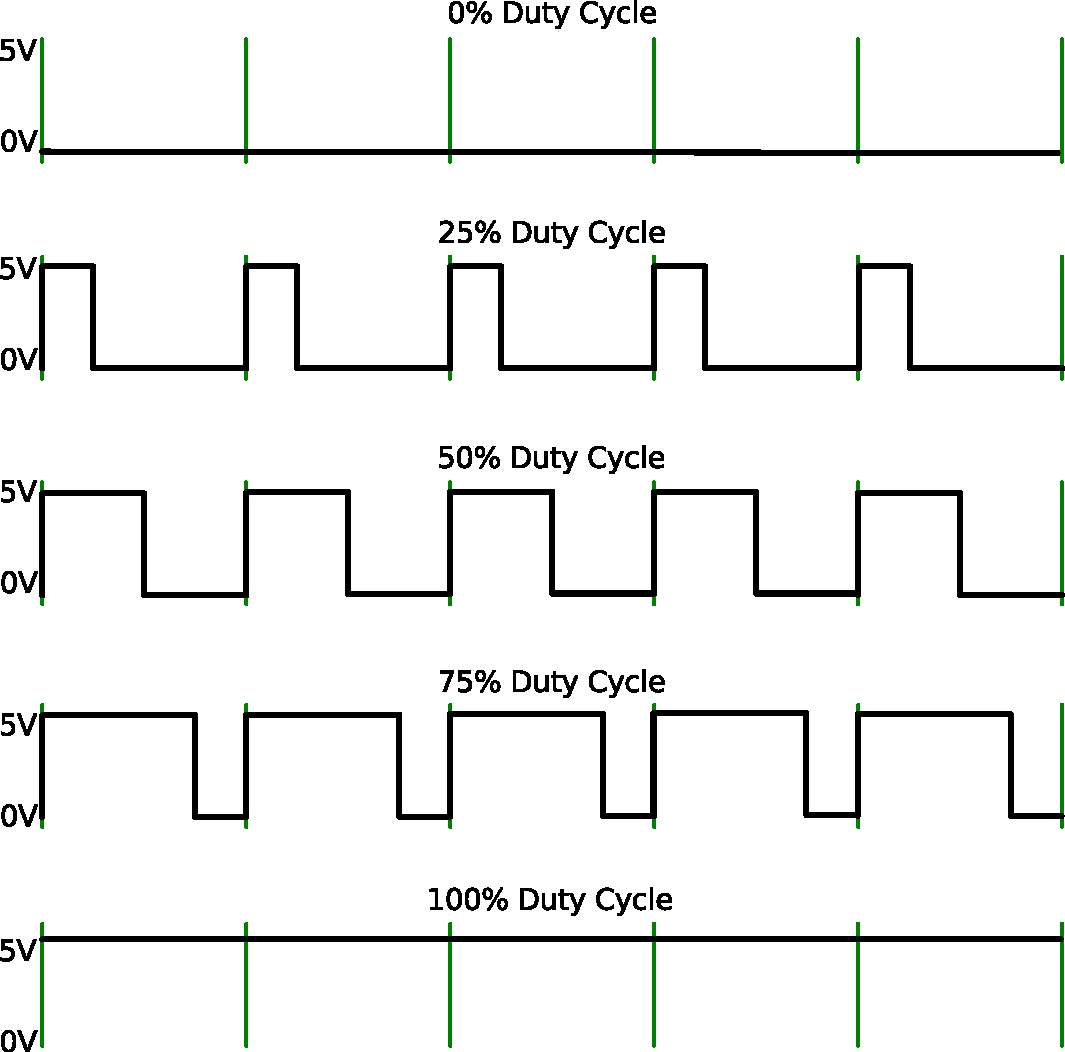
\includegraphics[height=0.8\textheight]{./img/pwmmeu.pdf}
\end{figure}
\end{frame}
%-----------------------------------------------------------------------------

%-----------------------------------------------------------------------------
\begin{frame}{Modulação por largura de pulso (PWM)}
\begin{figure}
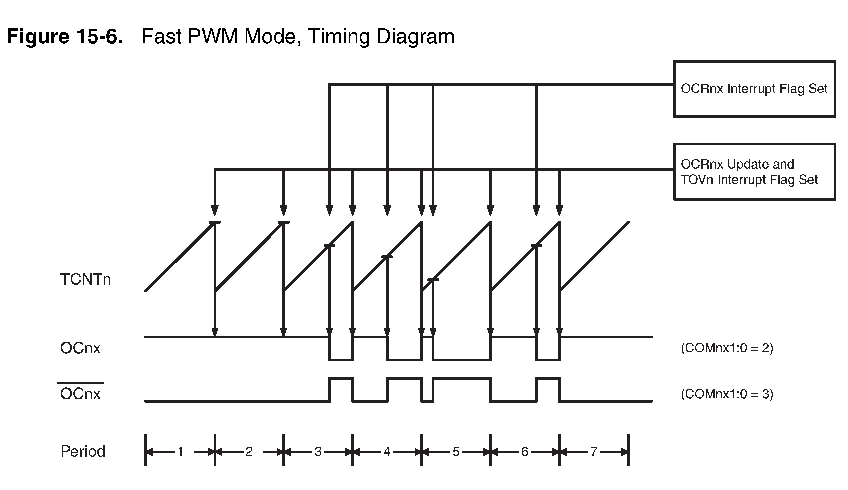
\includegraphics[width=\textwidth]{./img/pwm2.pdf}
\end{figure}
\end{frame}
%-----------------------------------------------------------------------------

%-----------------------------------------------------------------------------
\begin{frame}{Modulação por largura de pulso (PWM)}
\begin{figure}
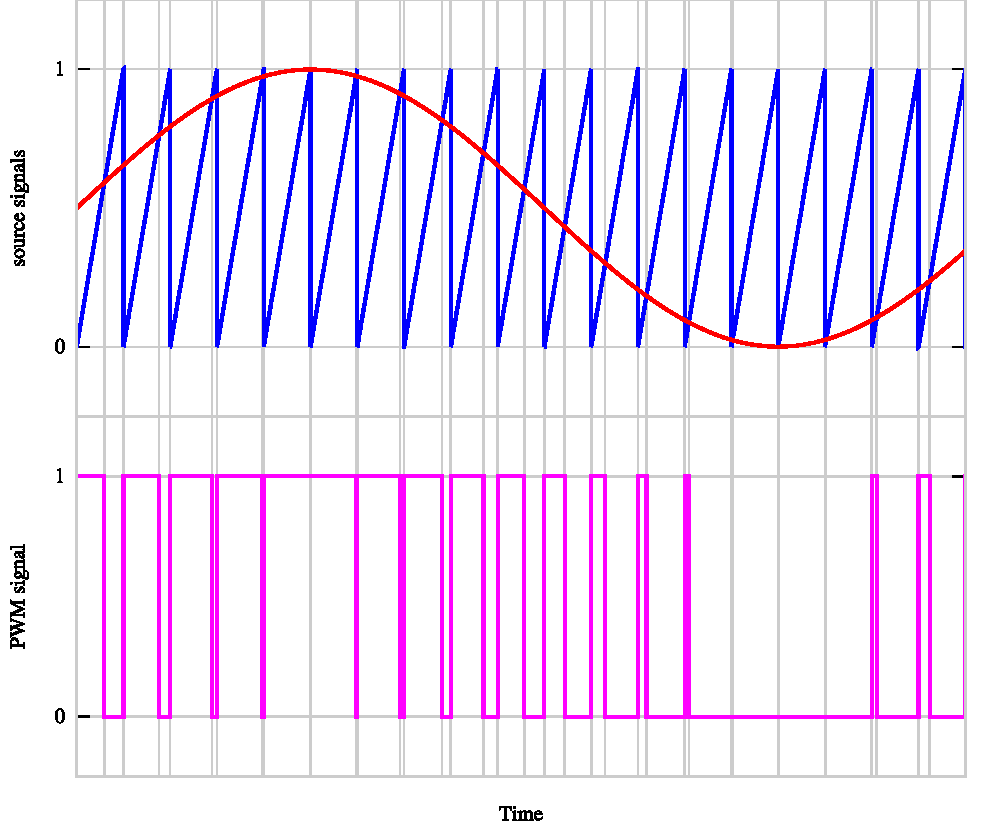
\includegraphics[width=0.8\textwidth]{./img/Pwm.pdf}
\end{figure}
\end{frame}
%-----------------------------------------------------------------------------

%-----------------------------------------------------------------------------
\begin{frame}{Modulação por largura de pulso (PWM)}
Características de PWM no ATmega328P:
\begin{itemize}
  \item 6 canais de saída.
  \item Modos de operação: \emph{Fast} e \emph{Phase Correct}.
  \item Pré-escalonador.
%  \item Compare Match output mode.
  \item 2 contadores de 8 bits e 1 de 16 bits.
%  \item Período fixo e variável.
  \item Interrupção por transbordamento.
\end{itemize}
\end{frame}
%-----------------------------------------------------------------------------

%-----------------------------------------------------------------------------
\begin{frame}{Modulação por largura de pulso (PWM)}
Frequências de operação de um contador de 8 bits:
\begin{center}
\begin{tabular}{crrrr}
\toprule
\toprule
\footnotesize{pré-escalonador} &
\footnotesize{$f_\text{incr}$ (KHz)} &
\footnotesize{$f_\text{overflow}$ (Hz)}  \\
\midrule
\rowcolor{LightCyan}
1 & 16.000 & 62.500 \\
8 & 2.000 & 7.812 \\
32 & 500 & 1.953 \\
64 & 250 & 976 \\
128 & 125 & 488 \\
256 & 62,5 & 244 \\
1024 & 15,625 & 61 \\
\bottomrule
\end{tabular}
\end{center}
\end{frame}
%-----------------------------------------------------------------------------

%-----------------------------------------------------------------------------
\begin{frame}{Modulação por largura de pulso (PWM)}
Parâmetros escolhidos:
\begin{itemize}
  \item \emph{Fast PWM}.
  \item Contador de 8 bits.
  \item Pré-escalonador igual a 1.
  \item Frequência de \emph{overflow}: 16~MHz / 1 / $2^8$ = 62.500~Hz.
  \item Taxa de geração de amostras: 31.250~Hz.
\end{itemize}
\end{frame}
%-----------------------------------------------------------------------------
\subsection{Processamento}


%-----------------------------------------------------------------------------
\begin{frame}[fragile]{Acoplamento de entrada e saída}
\begin{lstlisting}
// 1. leitura da entrada: ADC
x[ind] = ADCH;

// 2. escrita na saida: PWM
OCR2A = y[(ind-MIN_DELAY)&(BUFFER_SIZE-1)];

// 3. sinalizacao de um novo bloco de amostras
if ((ind & (BLOCK_SIZE - 1)) == 0) {
  rind = (ind-BLOCK_SIZE) & (BUFFER_SIZE-1);
  dsp_block = true;
}

// 4. incremento do indice de leitura/escrita
ind++;
ind &= BUFFER_SIZE - 1;

// 5. inicia uma nova conversao ADC
sbi(ADCSRA,ADSC); 
\end{lstlisting}
\end{frame}
%-----------------------------------------------------------------------------


%-----------------------------------------------------------------------------
\begin{frame}[fragile]{Implementação}
Detalhes importantes para implementar o sistema:
\begin{itemize}
  \item ADC:
  \begin{itemize}
    \item Valor do pré-escalonador.
    \item Alinhamento do resultado (resolução).
    \item Valor de referência.
    \item Pino de entrada.
  \end{itemize}
  \item PWM:
  \begin{itemize}
    \item Modo \emph{Fast PWM}.
    \item Valor do pré-escalonador.
    \item Pino de saída.
  \end{itemize}
  \item Compilação: \texttt{avr-gcc}, \texttt{avr-g++}.
  \item Monitoramento serial: \texttt{minicom}.
\end{itemize}
\end{frame}
%-----------------------------------------------------------------------------


%-----------------------------------------------------------------------------
\begin{frame}{Memória}
Limites da Memória:
\begin{itemize}
  \item 2~Kb de SRAM para dados.
  \item Uma tabela com 512 bytes ocupa $\frac{1}{4}$ da memória!
  \item Buffer máximo de 2.000 amostras.
\end{itemize}
\end{frame}
%-----------------------------------------------------------------------------



